
%Move 1.2.2 Distinction of Approaches to here.

\subsection{Solution Diversity in the Multi objective Paradigm}


We made a choice in algorithm design that would promote diversity of optimised model solutions.

%in the multi objective paradigm.

In an eight objective error function there are eight different ways for one score to be significantly better than the rest of the scores, and many different ways for the sum of two or more scores to be significantly better than one of the error scores. Although you are expecting diverse solutions its often practical to take just pick the most optimal model solution.

But if you were optimizing models that you intend to use to populate brain network simulations, you may actually benefit from multiple parameter sets for each cell.

In order to promote diversity in the models of particular cell types we took on each model parameter and calculated the unique current injection value that would cause that cell to fire a single spike. 

\subsection{Rheobase as a Soft Constraint}
One major difference in our methodological approach was to promote diversity among candidate solutions to optimisation problems. 
of rheobase 
%\graphicspath{figures}
\begin{figure}    
\begin{center}
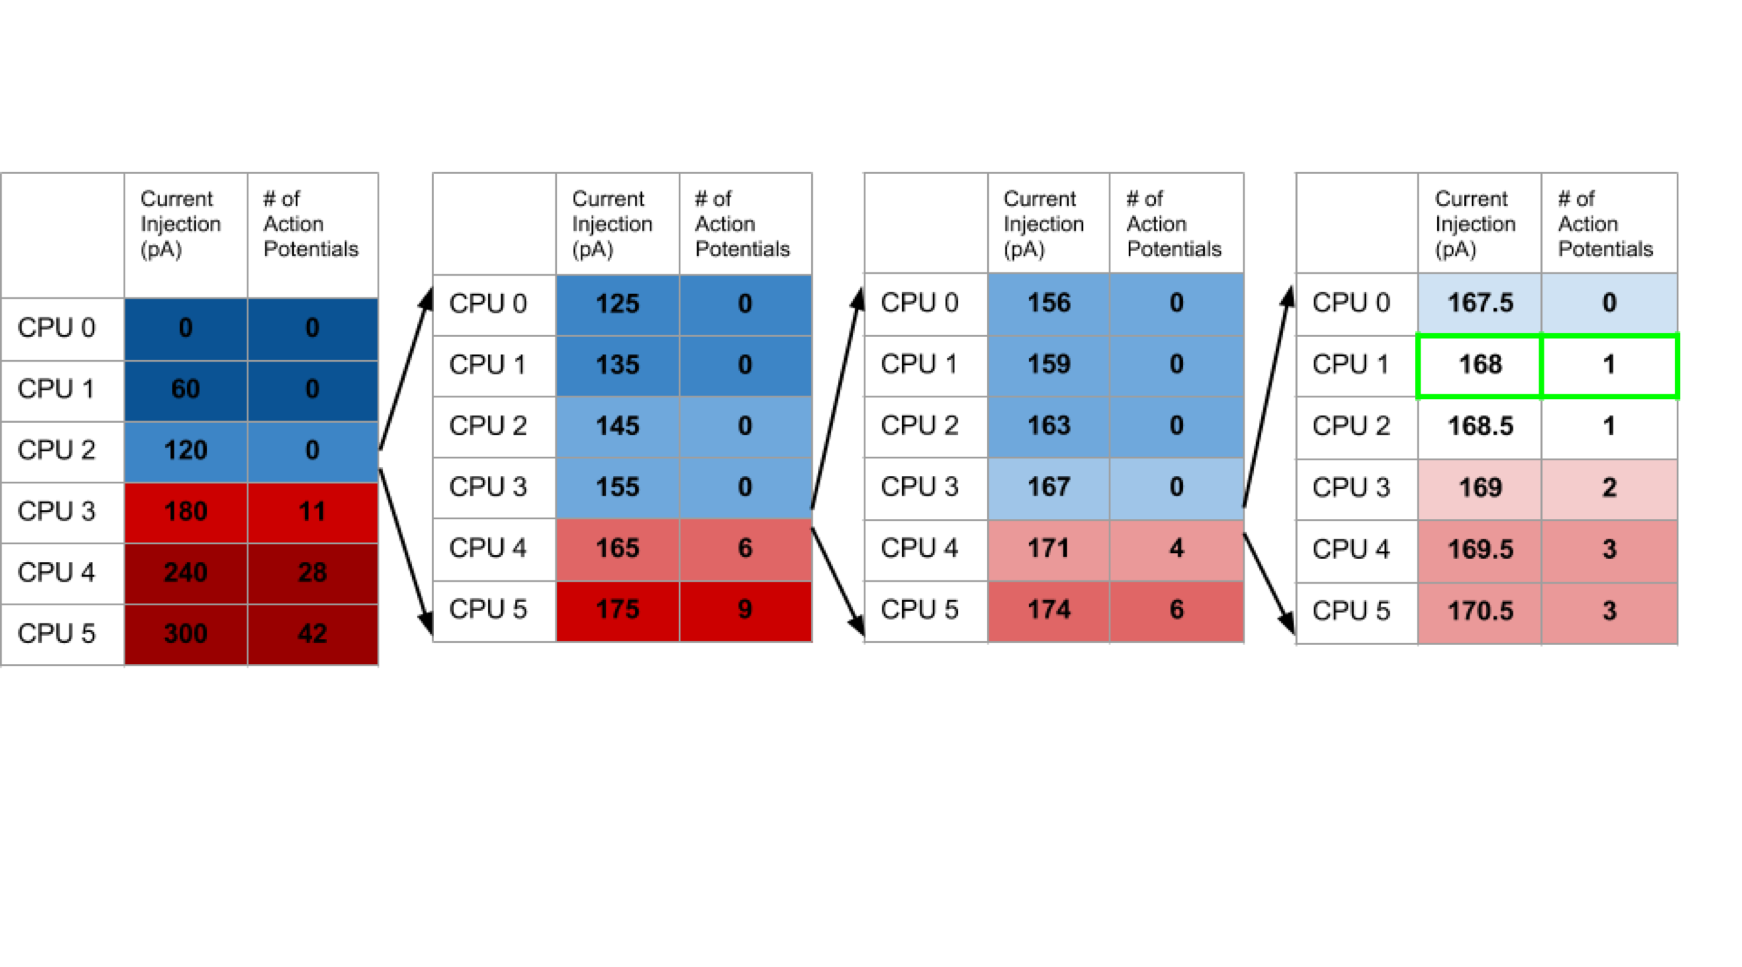
\includegraphics[width=0.7\linewidth]{chapters/figures/rheobase_algorithm.png}
\caption{We developed a generic algorithm which took models, and found the minimal current injection value that would cause only one spike. The normal structure of this algorithm is a binary search, however we modified the algorithm so it would map onto multiple processors at once. This lead to significant speed ups for multicompartment NEURON models}

\end{center}
\end{figure}  

\begin{figure}    
\begin{center}
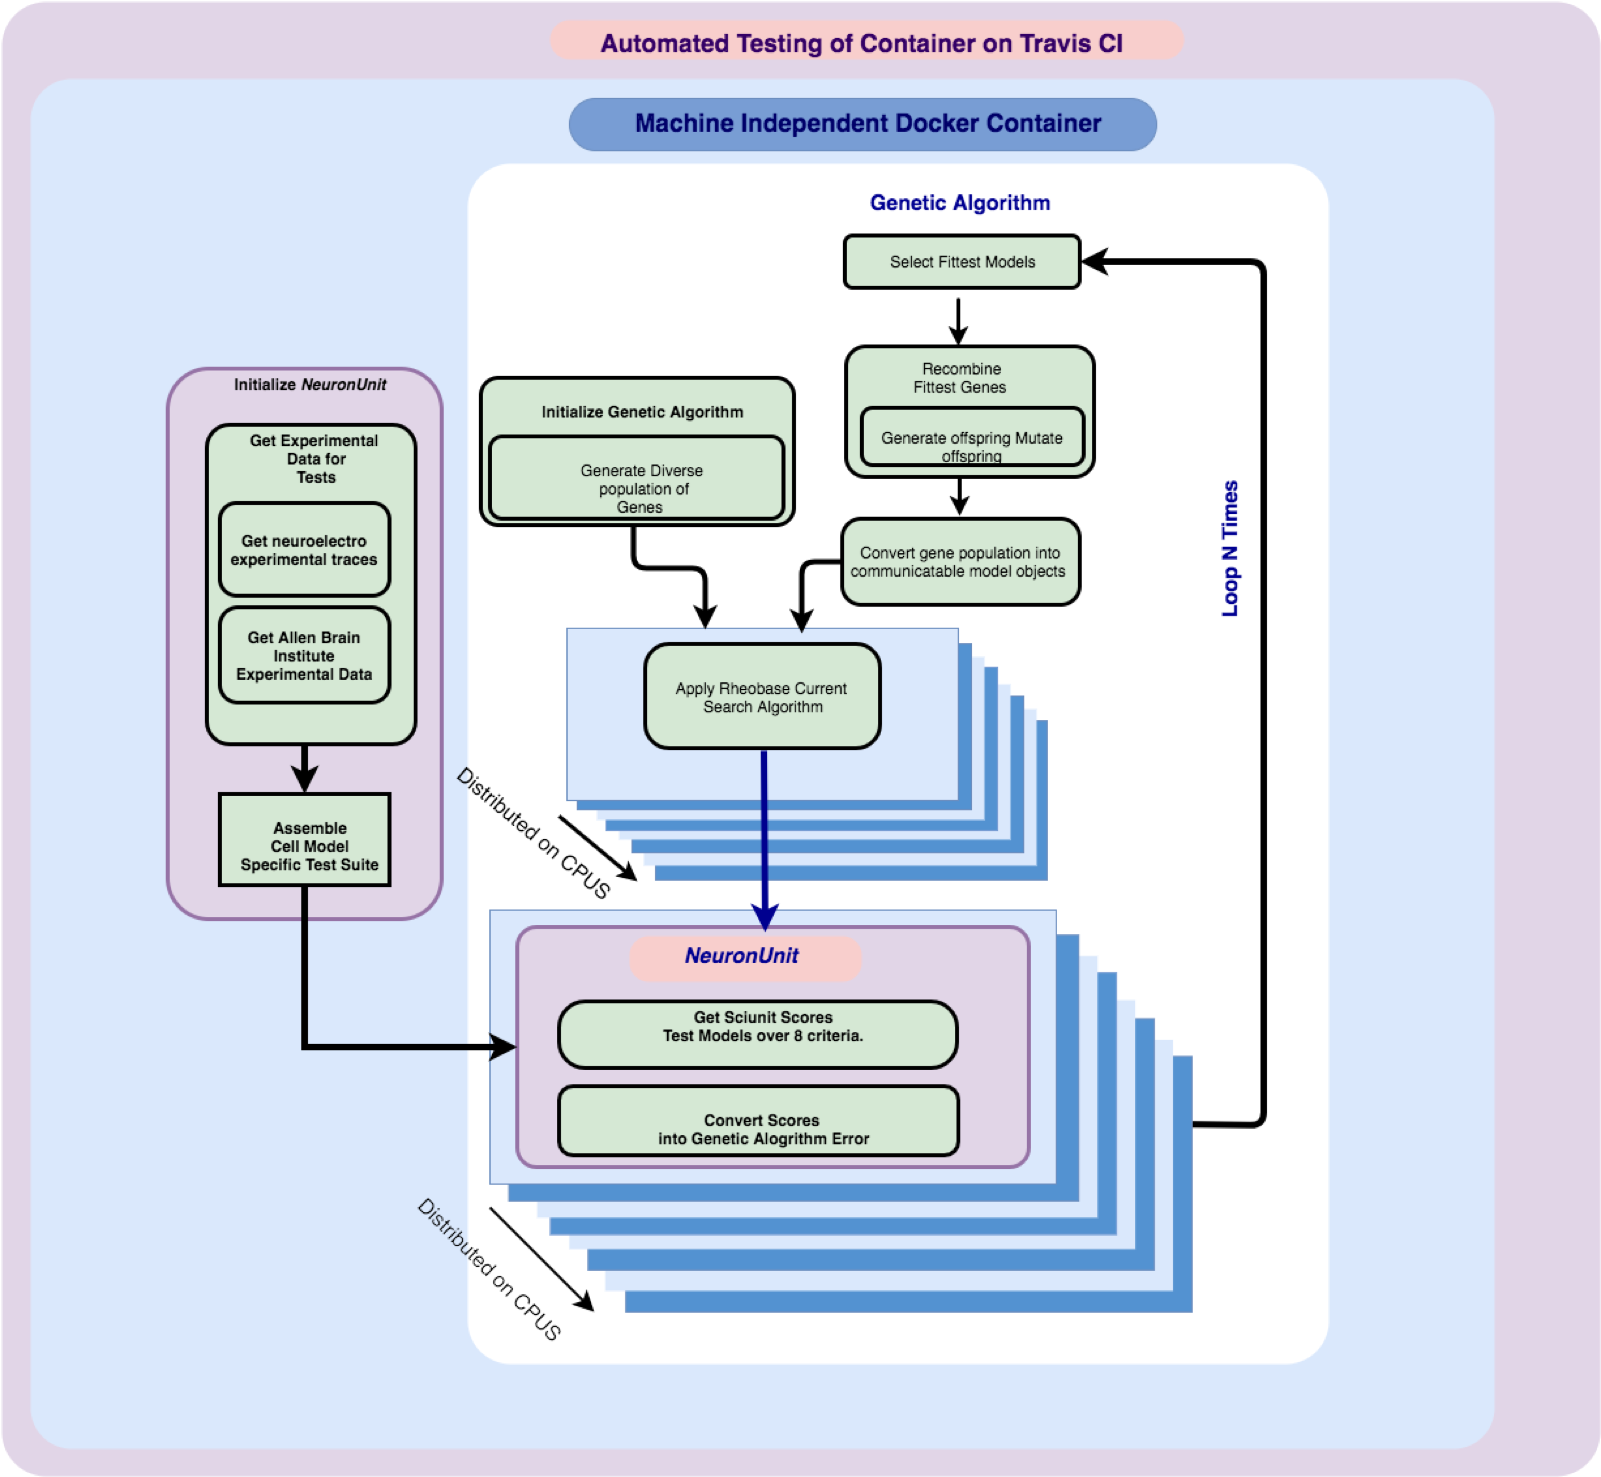
\includegraphics[width=0.7\linewidth]{chapters/figures/software_architecture.png}
\caption{In the process of performing the analysis in this work, we expanded an existing neuron model optimisation frame work BluePyOpt \cite{bluepyopt}, by adding in workflows to handle different and elaborate constraint functions and different and elaborate models. and found the minimal current injection value that would cause only one spike. The normal structure of this algorithm is a binary search, however we modified the algorithm so it would map onto multiple processors at once. This lead to significant speed ups for multicompartment NEURON models}

\end{center}
\end{figure}



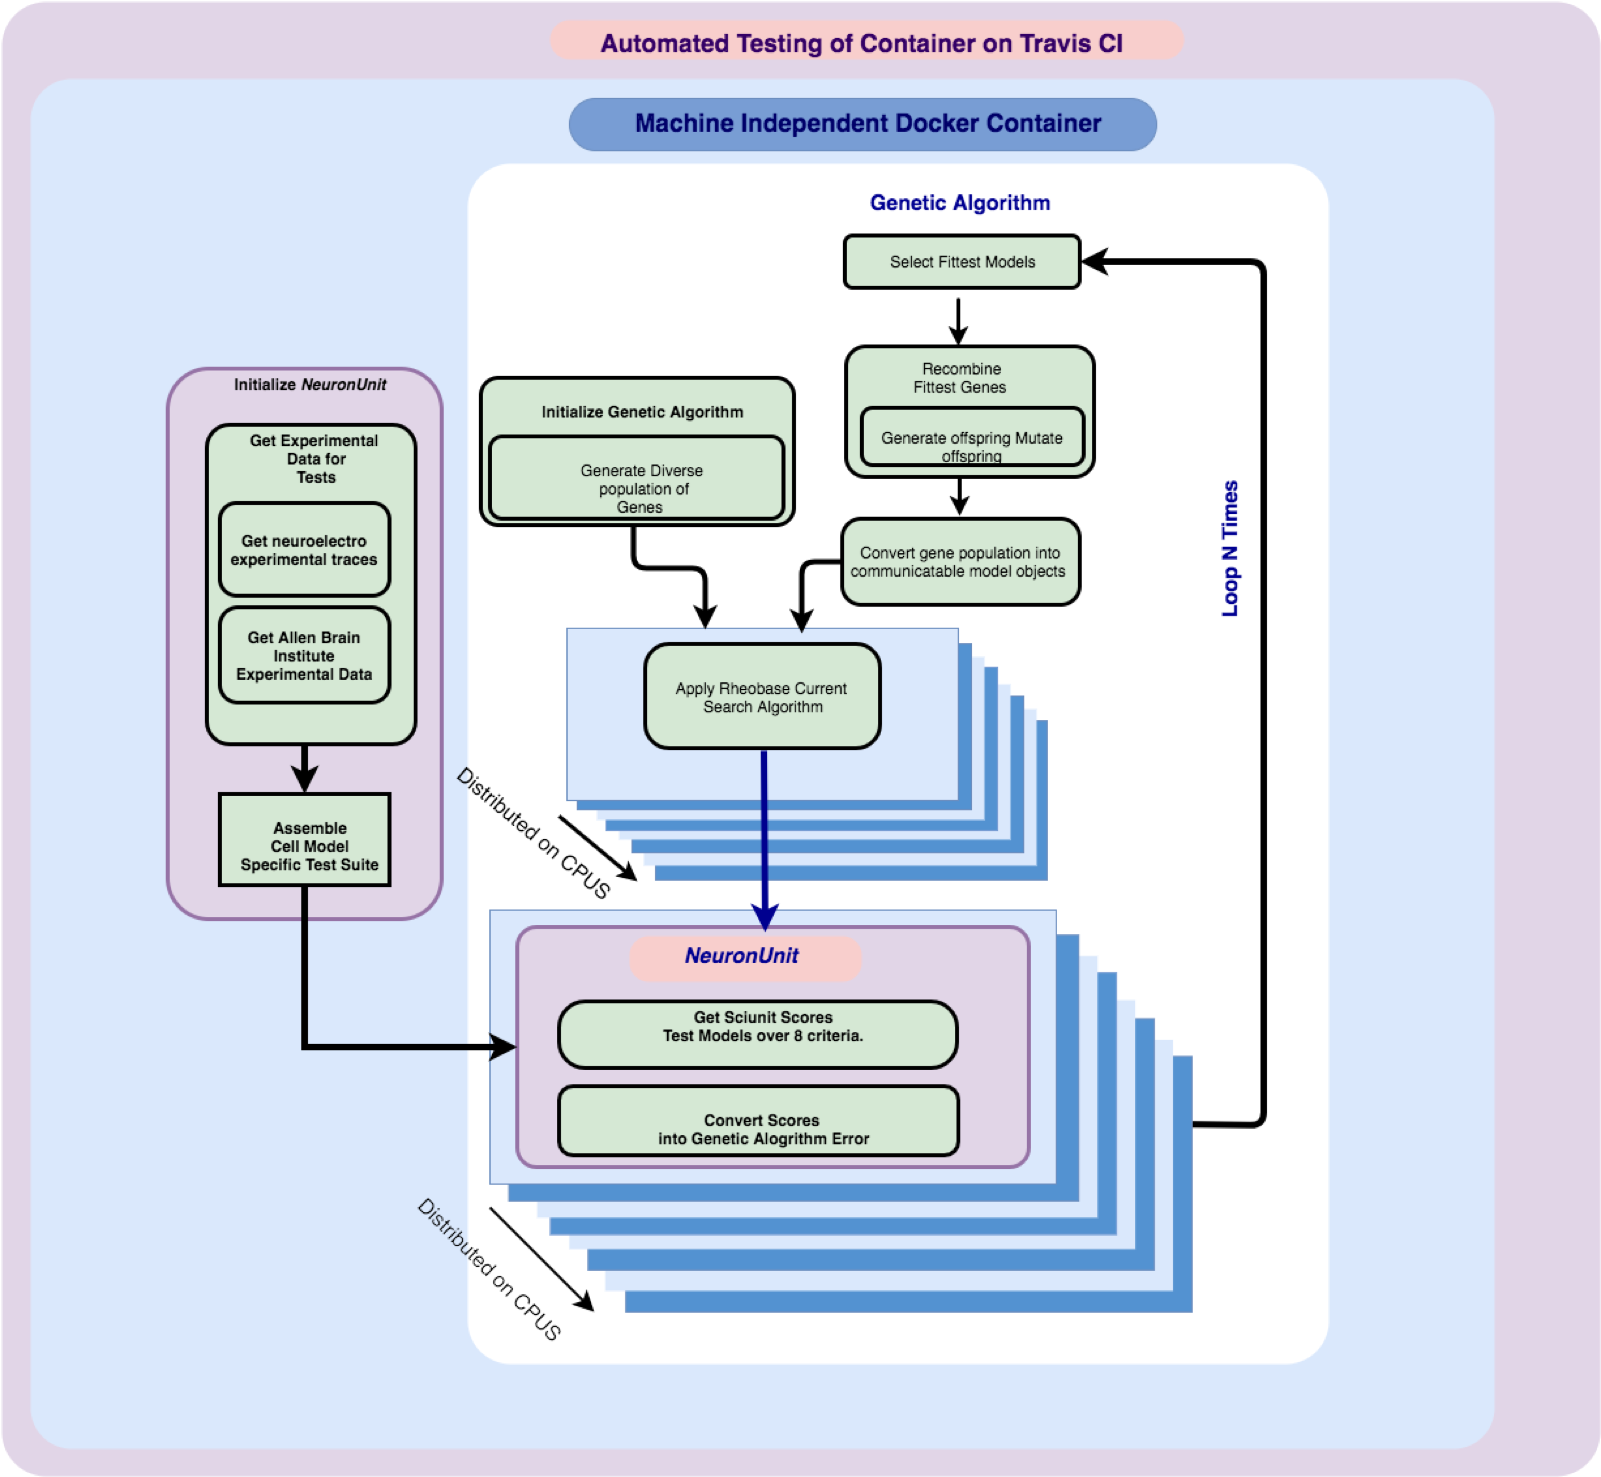
\includegraphics[width=0.7\linewidth]{chapters/figures/software_architecture}

